\documentclass[main.tex]{subfiles}
\renewcommand{\epsilon}{\varepsilon}
\begin{document}

\section{Introduction}
\emph{blabla ,les centrales nucléaire c'est 1GW , avec des machines synchrones. Les MCC sont pas utilisé en forte puissance. on préfère utiliser une machine synchrone ou une machine asynchrone (plus simple, moins cher,etc)}
La machine asynchrone fonctionne en moteur ou en alternateur.

Premier brevet déposé en 1888 par Nicolas Tesla.

Utilisation des différentes technologies de moteur (brushless, bobinés) en automobile et industrie (80\% des moteur de l'industrie sont des machines asynchrones)


\section{Principe de la machine asynchrone}
en anglais on parle de \emph{Induction Motor}.
On génère un champ magnétique tournant au stator
Le courant électrique est induit dans le rotor , pas besoin de mettre des balais ou de bobinage au rotor.

\subsection{Le stator triphasé}
\subsubsection{Champs tournant}

On a le schéma suivant, $n$ spires sont parcourues par un courant $i_{sa}$.
\begin{figure}[H]
  \centering
  \begin{subfigure}{0.5\textwidth}
  \centering
  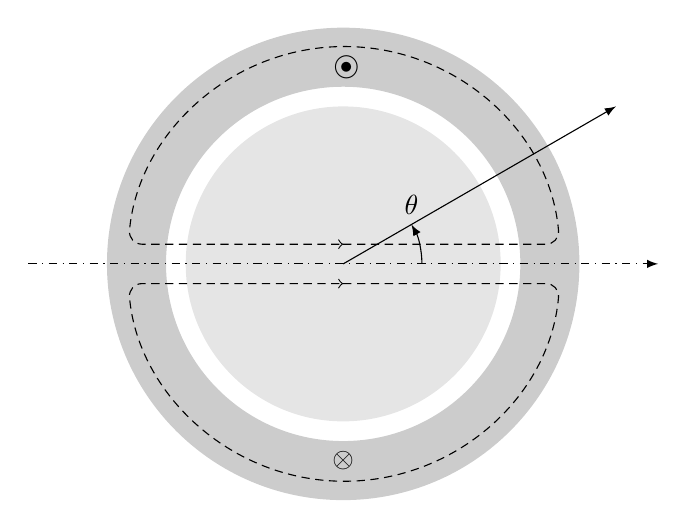
\begin{tikzpicture}
    \fill[gray!40,even odd rule] (0,0) circle(2.25) circle (3);
    \fill[gray!20] (0,0) circle (2);
    \draw[-latex,dash dot] (-4,0) -- (4,0);
    \draw[-latex] (0,0) -- ++(30:4);
    \draw[-latex] (1,0) arc(0:30:1) node[above]{$\theta$};
    \draw (0,2.5)node[]{\small$\bigcirc\hspace{-0,75em}\bullet$}
          (0,-2.5)node[]{{$\otimes$}};
    \draw[->,densely dashed, thin,rounded corners=5pt] (0, 0.25) -- (2.75, 0.25)  arc[start angle=5, end angle=175, radius=2.75]-- (0, 0.25);
    \draw[->,densely dashed,thin,rounded corners=5pt] (0, -0.25) -- (2.75, -0.25)  arc[start angle=-5, end angle=-175, radius=2.75] -- (0, -0.25);
  \end{tikzpicture}
  \subcaption{Schéma du stator (monophasé)}
\end{subfigure}%
\begin{subfigure}{0.5\textwidth}
  \centering
  \begin{tikzpicture}
    \begin{axis}
      [axis lines = middle,
      xlabel=$\theta$,ylabel=$\epsilon_s$,
      xmax=3,xmin=-3,ymin=-1.5,ymax=1.5,
      samples=41,
      xtick={-1,1},ytick=\empty,
      xticklabels={$-\frac{\pi}{2}$, $\frac{\pi}{2}$}]
      \addplot+[no marks] plot coordinates {(-2,-1) (-1,-1) (-1,1) (1,1) (1,-1) (2,-1)};
      \addplot+[no marks,color=black, dashed] {cos(pi*deg(x)/2)};
    \end{axis}
  \end{tikzpicture}
  \subcaption{Force magnétomotrice $\epsilon_s$}
\end{subfigure}
\caption{Champ tournant dans le stator}
\end{figure}
Avec le théorème d'ampère on a :

\begin{align*}
  \oint \vec{H}.\vec{dl} &= n_s i_s\\
  \underbrace{ \int H.dl}_{H_{fer}} &+ \underbrace{2H_c e}_{H_e} = n_s i_s\\
  \intertext{Or on a: }
  H_{mat.fer} &\ll H_{entrefer}
                \intertext{Donc on a la force magnétomotrice}
                \Aboxed{\epsilon_s = H_ee =\frac{n_si_s}{2}}
\end{align*}
On peux donc tracer :


La répartition des fils autour du rotor influe sur l'allure de la force magnétomotrice. Par exemple pour une répartition uniforme de $n/3$ spires par encoche :
\begin{figure}[H]
  \centering
  \begin{subfigure}[b]{.5\textwidth}
  \centering
  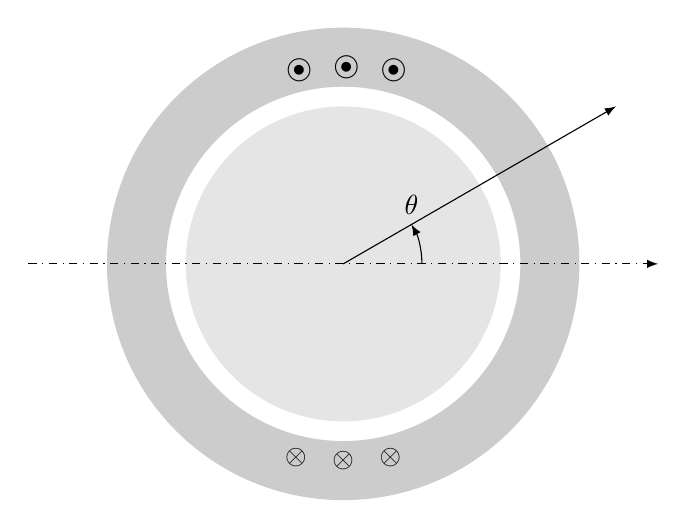
\begin{tikzpicture}
    \fill[gray!40,even odd rule] (0,0) circle(2.25) circle (3);
    \fill[gray!20] (0,0) circle (2);
    \draw[-latex,dash dot] (-4,0) -- (4,0);
    \draw[-latex] (0,0) -- ++(30:4);
    \draw[-latex] (1,0) arc(0:30:1) node[above]{$\theta$};
    \draw (0.6,2.46)node[]{\small$\bigcirc\hspace{-0,75em}\bullet$}
          (0.6,-2.46)node[]{{$\otimes$}};
    \draw (0,2.5)node[]{\small$\bigcirc\hspace{-0,75em}\bullet$}
          (0,-2.5)node[]{{$\otimes$}};
    \draw (-0.6,2.46)node[]{\small$\bigcirc\hspace{-0,75em}\bullet$}
          (-0.6,-2.46)node[]{{$\otimes$}};
  \end{tikzpicture}
  \subcaption{Schéma du stator (monophasé)}
\end{subfigure}%
\begin{subfigure}[b]{0.5\linewidth}
  \centering
  \begin{tikzpicture}
    \begin{axis}
      [axis lines = middle,
      height=7.6cm,
      xlabel=$\theta$,ylabel=$\epsilon_s$,
      xmax=3,xmin=-3,ymin=-1.5,ymax=1.5,
      samples=41,
      xtick={-1,1},ytick=\empty,
      xticklabels={$-\frac{\pi}{2}$, $\frac{\pi}{2}$}]
      \addplot+[no marks] plot coordinates {(-2,-1) (-1.5,-1) (-1.5,-0.5)   (-1,-0.5) (-1,0.5)(-0.5,0.5) (-0.5,1)  (0.5,1) (0.5,0.5) (1,0.5)(1,-0.5) (1.5,-0.5) (1.5,-1)(2,-1)};
      \addplot+[no marks,color=black, dashed] {cos(pi*deg(x)/2)};
    \end{axis}
  \end{tikzpicture}
  \subcaption{Force magnétomotrice $\epsilon_s$}
\end{subfigure}
\caption{Approximation sinusoïdale du champ tournant}
\end{figure}

en répartissant les bobinage sur le rotor de manière sinusoïdales , on peux générée une force magnétomotrice sinusoïdale également.

\begin{rem}
On utilise despetit fils pour éviter l'effet de peau en alternatif, mais cela augmente la resistivité et la puissance dissipée par effet joule, rien n'est parfait.
\end{rem}

En utilisant un courant $i_s$ alternatif (à la pulsation $\omega$) on a une onde pulsante:
\[
  \epsilon_s =\frac{n_si_{max}}{2}cos(\omega t)
\]

\begin{figure}[H]
  \centering
  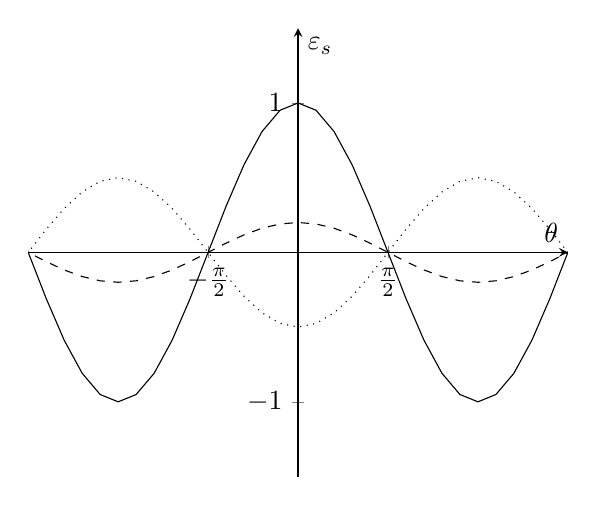
\begin{tikzpicture}
    \begin{axis}
      [axis lines = middle,
      xlabel=$\theta$,ylabel=$\epsilon_s$,
      xmax=3,xmin=-3,ymin=-1.5,ymax=1.5,
      samples=51,
      xtick={-1,1},ytick={},
      xticklabels={$-\frac{\pi}{2}$, $\frac{\pi}{2}$}]
      \addplot+[no marks,color=black] {cos(pi*deg(x)/2)};
      \addplot+[no marks,color=black, dashed] {0.2*cos(pi*deg(x)/2)};
      \addplot+[no marks,color=black, dotted] {-0.5*cos(pi*deg(x)/2)};
    \end{axis}
  \end{tikzpicture}
  \caption{Évolution d'une onde pulsante en fonction du temps}
\end{figure}


Dans le cas triphasé on répartis les enroulements de manière sinusoïdales (seul un tour de bobinage est représenté) parcourus par $i_{sa} ,i_{sb},i_{sc}$ :
\[
  \begin{cases}
    i_{sa}(t)=I\sqrt{2}\cos(\omega t) \\
    i_{sb}(t)=I\sqrt{2}\cos(\omega t+ \frac{2\pi}{3}) \\
    i_{sc}(t)=I\sqrt{2}\cos(\omega t-\frac{2\pi}{3})
  \end{cases}
  \text{ Soit }
  \begin{cases}
    \epsilon_{sa}(t) = \frac{n_si_s(t)}{2} \cos(\theta) \\
    \epsilon_{sb}(t) = \frac{n_si_s(t)}{2} \cos(\theta-\frac{2\pi}{3}) \\
    \epsilon_{sc}(t) = \frac{n_si_s(t)}{2} \cos(\theta+\frac{2\pi}{3}) \\
  \end{cases}
\]

\begin{figure}[H]
  \centering
  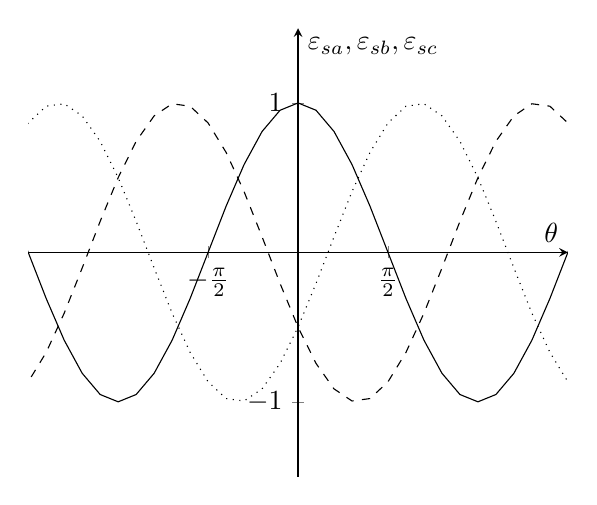
\begin{tikzpicture}
    \begin{axis}
      [axis lines = middle,
      xlabel=$\theta$,ylabel=${\epsilon_{sa},\epsilon_{sb},\epsilon_{sc}}$,
      xmax=3,xmin=-3,ymin=-1.5,ymax=1.5,
      samples=51,
      xtick={-1,1},ytick={},
      xticklabels={$-\frac{\pi}{2}$, $\frac{\pi}{2}$}]
      \addplot+[no marks,color=black] {cos(pi*deg(x)/2)};
      \addplot+[no marks,color=black, dashed] {cos(pi*deg(x)/2+120)};
      \addplot+[no marks,color=black, dotted] {cos(pi*deg(x)/2-120)};
    \end{axis}
  \end{tikzpicture}
  \caption{Forces magnétomotrices en triphasé}
\end{figure}
Alors la force magnétomotrice totale vaut:
\begin{align*}
  \epsilon_s &=\epsilon_a +\epsilon_b+\epsilon_c \\
      &= \frac{n_sI\sqrt{2}}{2}\left(
        \cos(\theta)\cos(\theta)   + \cos(\omega t-\frac{2\pi}{3})\cos(\theta-\frac{2\pi}{3})
 +\cos(\omega t-\frac{2\pi}{3})\cos(\theta-\frac{2\pi}{3})
        \right)\\
       \Aboxed{ &= \frac{3n_sI}{\sqrt{2}} \cos(\theta-\omega t)}
\end{align*}

On a créer un champ tournant , avec trois bobinage , le module de la force magnétomotrice est constant , son argument balaye tout l'espace.

\subsection{Rotor à une spire en court circuit}
\begin{figure}[H]
  \begin{subfigure}[b]{.5\textwidth}
  \centering
  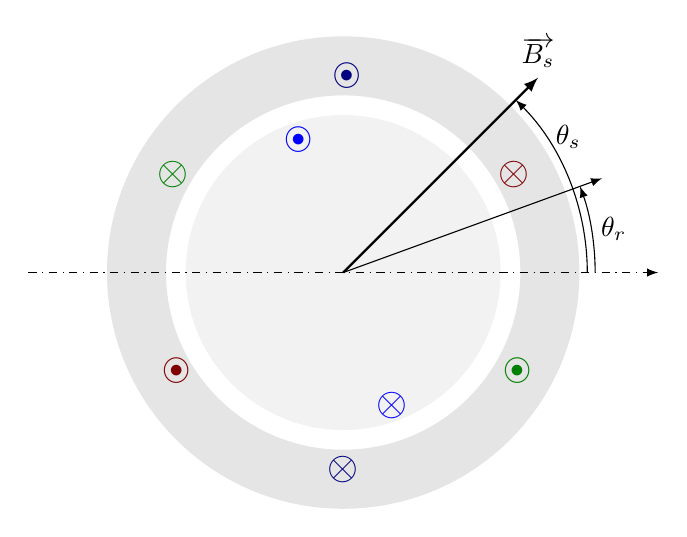
\begin{tikzpicture}
    \fill[gray!20,even odd rule] (0,0) circle(2.25) circle (3);
    \fill[gray!10] (0,0) circle (2);
    \draw[-latex,dash dot] (-4,0) -- (4,0);
    \draw
    (110:1.8)node[blue]{$\bigcirc\hspace{-0,75em}\bullet$}  (110:-1.8)node[blue]{{\Large$\otimes$}};
\draw
    (90:2.5)node[blue!50!black]{$\bigcirc\hspace{-0,75em}\bullet$} (90:-2.5)node[blue!50!black]{{\Large$\otimes$}}
    (210:2.5)node[red!50!black]{$\bigcirc\hspace{-0,75em}\bullet$} (210:-2.5)node[red!50!black]{{\Large$\otimes$}}
    (330:2.5)node[green!50!black]{$\bigcirc\hspace{-0,75em}\bullet$} (330:-2.5)node[green!50!black]{{\Large$\otimes$}};
    \draw[-latex] (0,0) -- (20:3.5) ;
    \draw[-latex] (3.2,0) arc(0:20:3.2) node[midway,right]{$\theta_r$};
    \draw[thick,-latex] (0,0) -- (45:3.5)node[above]{$\overrightarrow{B_s}$};
    \draw[-latex] (3.1,0) arc(0:45:3.1) node[near end, right]{$\theta_s$};
  \end{tikzpicture}
  \subcaption{Disposition du rotor (monophasé)}
\end{subfigure}%
\begin{subfigure}[b]{.5\textwidth}
  \centering
  \begin{circuitikz}
    \draw (0,0) to[V,v=$e$] ++(0,2) to[R,l=$R_r$] ++(0,2)-- ++(2,0) |-(0,0);
  \end{circuitikz}
  \caption{Schéma électrique du rotor en court circuit}
\end{subfigure}
\end{figure}
On a :
\begin{align*}
  e&= -\deriv[\Phi]{t} =R_r i_r
  &= -L\deriv[i_r]{t}+B.n_rS_r\deriv[\theta_s-\theta_r]{t}\sin(\theta_s-\theta_r)\\
\end{align*}
Pour $\theta_s=\omega_st$ , position du champs statorique et $\theta_r = \Omega t+ \theta_{r_0}$ ,position du champ rotorique on a:

\[
  e = -L\deriv[i_r]{t}+B.n_rS_r(\omega_s-\Omega)\sin((\omega_s-\Omega)t+\theta_{r_0})
\]

\subsection{Rotor à 3 spires en court circuit}
\begin{figure}[H]
  \centering
  \begin{subfigure}{0.5\textwidth}
  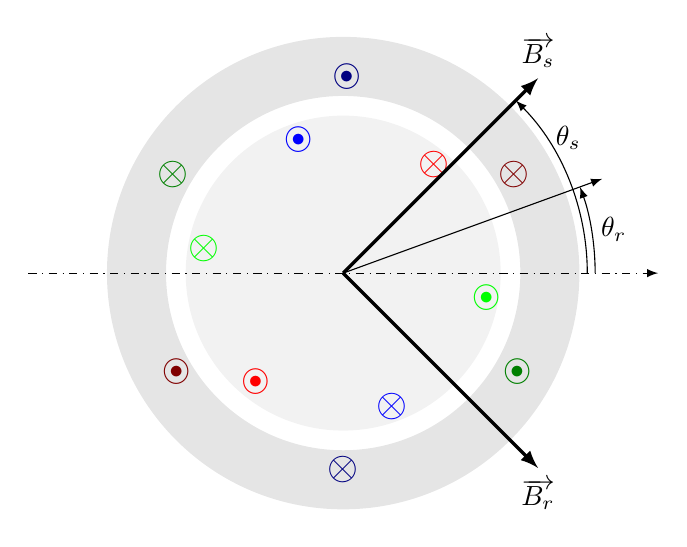
\begin{tikzpicture}
    \fill[gray!20,even odd rule] (0,0) circle(2.25) circle (3);
    \fill[gray!10] (0,0) circle (2);
    \draw[-latex,dash dot] (-4,0) -- (4,0);
    \draw
    (110:1.8)node[blue]{$\bigcirc\hspace{-0,75em}\bullet$}  (110:-1.8)node[blue]{{\Large$\otimes$}}
    (230:1.8)node[red]{$\bigcirc\hspace{-0,75em}\bullet$} (230:-1.8)node[red]{{\Large$\otimes$}}
    (350:1.8)node[green]{$\bigcirc\hspace{-0,75em}\bullet$} (350:-1.8)node[green]{{\Large$\otimes$}};

\draw
    (90:2.5)node[blue!50!black]{$\bigcirc\hspace{-0,75em}\bullet$} (90:-2.5)node[blue!50!black]{{\Large$\otimes$}}
    (210:2.5)node[red!50!black]{$\bigcirc\hspace{-0,75em}\bullet$} (210:-2.5)node[red!50!black]{{\Large$\otimes$}}
    (330:2.5)node[green!50!black]{$\bigcirc\hspace{-0,75em}\bullet$} (330:-2.5)node[green!50!black]{{\Large$\otimes$}};
    \draw[-latex] (0,0) -- (20:3.5) ;
    \draw[-latex] (3.2,0) arc(0:20:3.2) node[midway,right]{$\theta_r$};
    \draw[very thick,-latex] (0,0) -- (45:3.5)node[above]{$\overrightarrow{B_s}$};
    \draw[-latex] (3.1,0) arc(0:45:3.1) node[near end, right]{$\theta_s$};
        \draw[very thick,-latex] (0,0) -- (-45:3.5)node[below]{$\overrightarrow{B_r}$};
  \end{tikzpicture}
  \subcaption{Rotor triphasé}
\end{subfigure}%
\begin{subfigure}{0.5\textwidth}
  \begin{minipage}[h]{1.0\linewidth}
    On a:
    \begin{itemize}
    \item Vitesse de rotation de $\overrightarrow{B_s}$ : $\omega_s$
    \item Vitesse de rotation du rotor $\Omega$
    \item Vitesse de rotation de $\overrightarrow{B_s}$ dans le repère du rotor : $\omega_s-\Omega = \omega_r$
    \item Vitesse de rotation du champ $\overrightarrow{B_r}$ induit dans le rotor dans le repère du stator : $\omega_s$.
    \end{itemize}
    \begin{prop}
      Le champ induit dans le rotor et le champ du stator  tournent à la même vitesse, appelé \emph{la vitesse de synchronisme}
    \end{prop}
  \end{minipage}
\end{subfigure}
\end{figure}

\section{Modélisation de la machine asynchrone}
On considère une machine  triphasé au rotor et au stator à une paire de pôle:

\begin{figure}[H]
  \centering
  \begin{circuitikz}
    \draw[red] (0:2) node(As){} to[L,v=$V_{as}$,i^<=$i_{as}$,color=red] ++(0:2);
    \draw[red] (120:2)node(Bs){} to[L,v=$V_{bs}$,i^<=$i_{bs}$,color=red] ++(120:2);
    \draw[red] (240:2)node(Cs){} to[L,v=$V_{cs}$,i^<=$i_{cs}$,color=red] ++(240:2);
    \draw[dashed] (As) -- (0,0) (Bs) --(0,0) (Cs) --(0,0);

    \draw[blue] (35:0.) node(Ar){} to[L,v^=$V_{ar}$,i_<=$i_{ar}$,color=blue] ++(35:2);
    \draw[blue] (155:0.)node(Br){} to[L,v^=$V_{br}$,i_<=$i_{br}$,color=blue] ++(155:2);
    \draw[blue] (275:0.)node(Cr){} to[L,v^=$V_{cr}$,i_<=$i_{cr}$,color=blue] ++(275:2);
    \draw[dotted] (Ar) -- (0,0) (Br) --(0,0) (Cr) --(0,0);
    \draw (0,0) circle(4);
    \draw[dotted] (0,0) circle(2) (35:2) -- ++ (35:2);
    \draw[-latex] (4.1,0) arc(0:35:4.1) node[midway,right]{$\theta =\Omega t$};
  \end{circuitikz}
  \caption{Modèle électrique}

  \paragraph{Hypothèses}
  \begin{itemize}
  \item Alimentation sinus triphasé en Régime Permanent
  \item Rotor triphasé en court-circuit
  \item Couplage en étoile des enroulements équilibrés
  \item Fmm sinusoïdales, pas de saturation magnétiques
  \end{itemize}
\end{figure}

On note $\omega_s$ pulsation des courants statoriquen $\omega_r$ la pulsation des courants rotorique et $\Omega$ la pulsation mécanique de la machine.

\subsection{Mise en équation}
\subsubsection{Équation statorique}

Chaque phase du stator possède un couplage magnétique avec les autres phases du stator (mutuelle $M_s$) et avec les phases du rotor (mutuelle $M_0$).

On a  les équations suivantes  pour le stator:
\begin{align*}
  v_{as} &= R_s i_{as}(t)+\deriv[\Phi_{as}(t)]{t}\\
  \Phi_{as}(t) &= L_{s} i_{as} + M_s(i_{bs}+i_{bs}) +M_0 (\cos(\theta)i_{ar}(t)+\cos(\theta+\frac{2\pi}{3})i_{br}(t)+\cos(\theta-\frac{2\pi}{3})i_{cr}(t))\\
  \Phi_{as}(t) &= (L_s-M_s) i_{as}(t)+\frac{3M_0I_r}{\sqrt{2}}\cos(\theta+\omega_rt+\phi_r+\theta_0) \\
  \Phi_{as}(t) &= (L_s-M_s) i_{as}(t)+\frac{3M_0I_r}{\sqrt{2}}\cos(\omega_st+\phi_s)
\end{align*}
On en déduit donc (Dans le formalisme complexe de l'ARQS)
\[\boxed{
  \underline{V_{as}} = R_s \underline{I_s}+jL_{sc}\omega_s\underline{I_{as}}+j \frac{3}{2}M_0\omega_s\underline{I_r}
}\]
$I_r$ est à la pulsation $\omega_s$ !

\subsubsection{Équations rotoriques}

On fais les mêmes calculs pour le rotor :

\begin{align*}
  v_{ar}(t) &= R_ri_{ar}(t) + \deriv[\Phi]{t}\\
  \Phi_{ar}(t) &= (L_{r}-M_r) i_{ar} +M_0( \cos(\theta)i_{as}(t)+\cos(\theta+\frac{2\pi}{3})i_{br}(t)+\cos(\theta-\frac{2\pi}{3})i_{cr}(t))\\
  \Phi_{ar}(t) &= (L_{r}-M_r) i_{ar} +\frac{3M_0I_s}{\sqrt{2}} \cos(\Omega t-\omega_st+\theta_0-\phi_s) \\
  \Phi_{ar}(t) &= L_{rc} i_{ar} +\frac{3M_0I_s}{\sqrt{2}} \cos(\omega_rt +\phi_s')
\end{align*}

Donc on a dans le formalisme complexe de l'ARQS, avec le rotor en court-circuit:

\[\boxed{
  V_{ar} = R_rI_{ar}+jL_{rc}\omega_rI_{ar}+j\frac32 M_0\omega_rI_s =0}
\]

On pose alors le \emph{facteur de glissement:}

\[
  \boxed{g= \frac{\omega_s-\Omega}{\omega_s}=\frac{\omega_r}{\omega_s}}
\]


\subsubsection{Modèle par analogie}

Dans le cas d'une machine à simple alimentation(on étudie l'usage d'une machine à double alimentation dans la partie \ref{sec:MADA}) le rotor est en court circuit:

\[
  \frac{\underline{V_{ar}}}{g} = 0 = \frac{R_r}{g} + jL_{Rc}\omega_sI_{ar}+j\frac32 M_0 \omega_sI_s
\]

Le facteur de glissement permets d'exprimer toute les grandeurs comme évoluant à la fréquence statorique.

Il y a un couplage magnétique entre le stator et le rotor , et on peux construire un modèle équivalent,avec $L_{sc}$ et $L_{rc}$ les inductances cycliques du stator et du rotor.
\begin{figure}[H]
  \centering
  \begin{circuitikz}
    \draw (0,0) to[open,v=$V_s$] ++(0,2) to[R,l=$R_s$,i>=$I_s$]++(2,0)to[short] ++(1,0) to[L,l_=$L_{sc}$] ++(0,-2) -- ++(-3,0);
    \draw (4,0) to[L,l_=$L_{rc}$] ++(0,2)
    to[short,i=$I_r$] ++(2,0)
    to[R,l=$R_r/g$] ++(0,-2) to[short] ++(-2,0);
    \draw[latex-latex] (3,2.1) to[bend left] ++(1,0) node[above left]{$\frac{3}{2}M_0$};
  \end{circuitikz}
  \caption{Modèle électrique équivalent}
\end{figure}

Le couplage n'est pas parfait: $\frac{3}{2}M_0 < \sqrt{L_{sc}L_{rc}}$.

On fait l'analogie avec un transformateur parfait avec pertes :
% l_fuite= l_2
% sigma = 1 - M_c^2/(L_cs L_cr)
\begin{figure}[H]
  \centering
  \begin{circuitikz}
    \draw (0,0) node[gyrator](G){}
    (G.A1) -- ++(-1,0) coordinate(M) to[L,l_=$L_{sc}$] ++(0,-2) |- (G.A2)
    (G.B1) to[L,l=$l_{fuites}$] ++(2,0) to[R,l=$R_r/g$] ++ (0,-2) |- (G.B2)
    (M) to[R,l=$R_s$] ++(-2,0)
    (G.A2) --  ++(-3,0) to[open,v=$V_s$] ++(0,2);
\draw[latex-latex] (G.A1)++(0,0.2) to[bend left] ++(2,0) node[midway, above=1.5em]{$m$} ;
  \end{circuitikz}
  \caption{Modèle électrique équivalent}
\end{figure}

L'inductance de fuite est la pour témoigné des fuites des lignes de champs qui ne circulent pas dans le rotor.

Avec $m = \frac{M_0}{L_{sc}}$ et  $l_{fuites} = L_r-\frac{M_0^2}{L_1}$

On a donc l'impédance équivalente suivante à alimenter:

\begin{figure}[H]
  \centering
  \begin{tikzpicture}

    \draw (0,0) to[open,v=$V_s$] ++(0,2) to[R,l=$R_s$,i>=$I_s$]++(2,0)to[short] ++(1,0) coordinate(A) to[L,l^=$L_{sc}$] ++(0,-2) -- ++(-3,0);
    \draw [dotted] (2,2) to[R,l_=$R_{fs}$] ++(0,-2);
    \draw (A) to[L,l=$l_{fr}'$] ++(2,0) to[R,l=$R_r'/g$]++(0,-2) to[short] ++(-2,0);
  \end{tikzpicture}
  \caption{impédance équivalente au stator}
\end{figure}

Avec:
\begin{itemize}
\item $ l_{fr}' = \frac{l_{fuite}}{m^2} $
\item  $R_r' = \frac{R_r}{m^2}$.
\item $R_{fs}$ est ajoutable pour prendre en comptes les pertes fertes, qui pourrait alors être considérée linéaire.
\end{itemize}

\paragraph{Détermination des grandeurs du modèle équivalent:}

\begin{itemize}
\item $R_s$ :
  Essai en courant continu , on mesure la resistance des bobinages d'une phase du stator.
\item $L_{sc}/R_{fs}$:
  Essai à vide au synchronisme.\\
  Lors d'un essai au synchronisme, le champ tournant et le rotor tournent à la même vitesse. Le glissement g est nul et 1/g tend vers l'infini. Le modèle équivalent d'une phase de la machine devient :
  \begin{figure}[H]
    \centering
    \begin{circuitikz}

      \draw (0,0) to[open,v=$V_{s0}$] ++(0,2) to[R,l=$R_s$,i>=$I_{s0}$]++(2,0)to[short] ++(1,0) coordinate(A) to[L,l^=$L_{sc}$] ++(0,-2) -- ++(-3,0);
      \draw [dotted] (2,2) to[R,l_=$R_{fs}$] ++(0,-2);
    \end{circuitikz}
    \caption{Modèle au synchronisme}
  \end{figure}
  On mesure la puissance active $P_0$ et la puissance réactive $Q_0$ et les courants $I_{s0}$ et $V_{s0}$ on obtient les équations:

\[
  \begin{cases}
    P_0 = R_s I_{S0}^2+\frac{V'^2}{R_{fs}}\\
    Q_0 = \frac{V'^2}{L_{sc}\omega_s}\\
    V'  = V_{s0} \frac{R_{fs}L_{sc}\omega}{\sqrt{(R_sR_{fs})^2+(L_{sc}\omega(R_F+R_s))^2}}
  \end{cases}
\]

$R_S$ étant connue, on peut calculer les trois inconnues :
$R_f,L_{sc},V'$
Le courant $I_{s0}$ étant faible lors de l'essai au synchronisme, on peut généralement négliger la chute de tension due à la résistance statorique devant la tension $V_{s0}$. Les équations deviennent alors :
\[
  \begin{cases}
    P_0 = \frac{V_{s0}^2}{R_{fs}}\\
    Q_0 = \frac{V_{s0}^2}{L_{sc}\omega_s}\\
  \end{cases}
\]
Et on a :
\[
  \boxed{R_F = \frac{V_{s0}^2}{P_0}} \text{ et } \boxed{L_{sc}=\frac{V_{s0}^2}{Q_0\omega}}
\]

\item $l_{fuites}/R_r$ :
  Essai en nominal, on connait le glissement:

\end{itemize}

\subsection{Bilan de puissance}

\begin{align*}
  P_{transmise} &= \frac{R_r}{g}I_r^2 \\
 P_{Joules, rotor} &= R_r I_r^2 \\
 P_{meca} &= P_{transmise}-P_{joules} = R_rI_r^2(\frac{1}{g}-1)
\end{align*}

Dans le modèle équivalent on est a $\omega_s$. Or dans le rotor les courants sont à $\omega_r$. On a alors: $\omega_r =g\omega_s$ Soit
\[\boxed{
g =\frac{\omega_s-\omega}{\omega_s}
}\]



\begin{figure}[H]
  \centering
\begin{tikzpicture}[x=1pt,y=1pt]

  \begin{sankeydiagram}[
    sankey tot length=90pt,%
    sankey tot quantity=6,%
    sankey min radius=15pt,%
    sankey fill/.style={
      draw,line width=0pt,
      %fill,
      white,
    },
    sankey draw/.style={
      draw=black,
      line width=1pt,
      line cap=round,
      line join=round,
    },
    ]
    \sankeynodestart{6}{0}{Pa}{0,100};
    \node[left] at (Pa) {$P_a=3UI\cos{\phi}$};
    \sankeyadvance{Pa}{50pt}

    \sankeyfork{Pa}{5/Pa2,1/Pjs}
      \sankeyturn{Pjs}{-90}
      \sankeyadvance{Pjs}{15pt}
      \sankeynodeend{1}{-90}{Pjs}{Pjs}
      \node[below=1em] at (Pjs) {$p_{js}=3R_sI_s^2$};

      \sankeyadvance{Pa2}{60pt}
      \sankeyfork{Pa2}{4/Ptr,1/Pfs}
        \sankeyturn{Pfs}{-90}
        \sankeyadvance{Pfs}{30pt}
        \sankeynodeend{1}{-90}{Pfs}{Pfs}
         \node[below=1em] at (Pfs) {$p_{fs}$};
        \sankeyadvance{Ptr}{60pt}
        \sankeynodeend{4}{0}{Ptr}{Ptr}
        \node[left] at (Ptr) {$P_{tr}=C_{em}\omega_s$};

        \sankeyadvance{Ptr}{30pt}
        \sankeyfork{Ptr}{3/Pr,1/Pjr}
          \sankeyturn{Pjr}{-90}
          \sankeyadvance{Pjr}{30pt}
          \sankeynodeend{1}{-90}{Pjr}{Pjr}
          \node[below=1em] at (Pjr) {$p_{jr}=gP_{tr}$};
          \sankeyadvance{Pr}{70pt}
          \sankeynodeend{3}{0}{Pr}{Pr}
          \node[left] at (Pr) {$P_r=C_{em}p\Omega$};
          \sankeyadvance{Pr}{30pt}
          \sankeyfork{Pr}{2/Pu,1/Pmec}
            \sankeyturn{Pmec}{-90}
            \sankeyadvance{Pmec}{30pt}
            \sankeynodeend{1}{-90}{Pmec}{Pmec}
            \node[below=1em] at (Pmec) {$p_{mec}$};
            \sankeyadvance{Pu}{60pt}
            \sankeynodeend{2}{0}{Pu}{Pu}
            \node[right=1em] at (Pu) {$P_{u}$};
      \draw [
    line width=3pt,
    decoration={
        brace,
        mirror,
        amplitude=10pt,
        raise=10pt
    },
    decorate
    ] (-20,0) -- ++ (180,0) node[midway, below=1.5em]{Stator};
      \draw [
    line width=3pt,
    decoration={
      brace,
      amplitude=10pt,
        mirror,
        raise=10pt
    },
    decorate
    ] (170,0) -- ++ (190,0) node[midway, below=1.5em]{Rotor};



  \end{sankeydiagram}
\end{tikzpicture}
  \caption{Bilan de puissance}
\end{figure}


\begin{exemple}
  Pour une machine asynchrone , 400V/690V ,1.5kW ,1425 tr/min :
  \begin{enumerate}
  \item La machines est cablé en triangle pour un réseau 400V (entre phase ,230V phase-neutre). \\
    Dans le cas d'un réseau 690V on cablera en étoile.
  \item En continu on mesure entre deux phase $R=$\SI{3.8}{\ohm}. Quel est la valeur de $R_s$ ?
  \item Pour une machine à vide $Q_{0T}=$\SI{1100}{VAR}et $P_{OT}$=\SI{200}{W}. Quelle est la valeur de $L_{cs}$ et  de $R_{fs}$?
  \item Au point nominal on mesure $I=$\SI{2,9}{A};$P_T$=\SI{1500}{W}:$Q_T=$\SI{1300}{VAR}. Quelle est la valeur de $l_{fr}'$ et $R_r'$?
  \end{enumerate}
\end{exemple}
\subsection{Couple et puissance}

À partir du modèle déterminer précédement on a en terme valeur efficaces:
\[
  I_r = \frac{V_s}{\sqrt{\left(R_s+\frac{R_r'}{g}\right)^2+(l_{fuites}\omega_s)^2}}
\]


\subsubsection{Couple en fonction du glissement}

On étudie une MAS à $p$ paire de poles :

\[
\Omega =(1-g)\frac{\omega_s}{p}
\]

En faisant le bilan de puissance au rotor  on a :

\[
P_e = 3 \frac{R_r'}{g}I_r^2 = C_e \Omega
\]

On en déduit alors le couple électromagnétique. \emph{en négligeant la resistance du stator}:
\begin{align*}
 C_{em} &=   3 p \frac{V_s^2}{\omega_s} \frac{\frac{R_r'}{g}}{\left(\frac{R_r'}{g}\right)^2+(l_{fuites}\omega_s)^2}\\
    &= 3 p \frac{V_s^2}{\omega_s} \frac{1}{\left(\frac{g(l_f\omega_s)^2}{R_r'}\right) + \frac{R_r'}{g(l_f\omega_s)^2}}\\
    &= \frac{3p}{l_f}\frac{V_s^2}{\omega_s^2}\frac{1}{\left(\frac{g(l_f\omega_s)^2}{R_r'}\right)+\left(\frac{R_r'}{g(l_f\omega_s)^2}\right)}\\
        \Aboxed{&= 2C_{max}\frac{1}{\left(\frac{g}{g_{max}}\right)+\left(\frac{g_{max}}{g}\right)}}
\end{align*}
Avec
\[
  \begin{cases}
    C_{max} = \frac{3p}{2l_f}\frac{V_s^2}{\omega_s^2}\\
    g_{max} = \frac{R_r'}{l_f\omega_s}
  \end{cases}
\]

La courbe représentative de l'expression du couple en fonction du glissement possède une symétrie par rapport à l'origine :
\begin{figure}[H]
  \centering
  \begin{tikzpicture}
    \begin{axis}
      [axis lines =middle,
      width = 14cm, height=8cm,
      xmin =-1.2, xmax = 1.2,
      ymin = -2.5, ymax = 2.5,
      ylabel=$C_{em}$,xlabel = $g$,
      xtick = {-1,-0.1,0.1,1},
      xticklabels={-1,$-g_{max}$,$g_{max}$,1},
      ytick= {-2,2},
      yticklabels={$C_{max}$,$-C_{max}$},
      domain=-1.5:1.5,
      samples=100,
      ]
      \addplot[blue] {4/(0.1/x + x/0.1)};
    \end{axis}
  \end{tikzpicture}
  \caption{Couple en fonction du glissement}
\end{figure}

Avec la relation glissement vitesse on a:
% Ajout de la figure
\begin{figure}[H]
  \centering
  \includegraphics[width=0.7\textwidth]{Domaines_fonctionnement_MAs.png}
  \caption{Mode de fonctionnement de la MAS}
\end{figure}
---

\subsection{Alimentation par un onduleur}
\emph{merci wikipédia}
\bigskip

Les onduleurs les plus répandus sont les onduleurs MLI (à modulation de largeur d'impulsion) dont le mode de commande permet de garder le rapport U1/f constant et d'obtenir des courants quasiment sinusoïdaux. U1 étant la valeur efficace du fondamental.
\subsubsection{Commande en U/f}
\paragraph{Présentation}

En régime sinusoïdal, la conservation du rapport U/f permet au circuit magnétique d'être dans le même état magnétique quelle que soit la fréquence d'alimentation. Autrement dit, la forme du cycle d'hystérésis parcouru par le circuit magnétique reste identique quelle que soit f. Ainsi, lorsque la fréquence diminue, la valeur efficace du fondamental de la tension diminuant dans les mêmes proportions, il n'y a pas de risque de saturation du matériau magnétique.

Ceci a pour conséquence qu'une commande qui maintient U1/f constant, où U1 représente la valeur efficace du fondamental, permet de conserver la même courbe de couple en fonction du glissement pour n'importe quelle fréquence d'alimentation. Les autres harmoniques présents, multiples de 5 et 7, créent des couples pulsants dont la moyenne est nulle.

Pour cela, la machine asynchrone est alimentée par un onduleur délivrant une tension de fréquence f et dont la valeur efficace du fondamental V1 est telle que le rapport V1/f est maintenu constant

\paragraph{Mise en équation}

On reprend l'équation générale du couple :

:\[ C_{em}= \frac{3 p}{\mathcal{N}_r} \cdot \frac{V_S^2}{ \omega_S^2} \cdot  \frac{1}{\left(\frac{g \mathcal{N}_r \omega_S}{R_r^*}\right)+ \left(\frac{R_r^* }{g \mathcal{N}_r \omega_S }\right)} \,\]

On note $ C_{max} $le couple maximal.

\[ C_{max}=\frac{3 p}{2*\mathcal{N}_r} \cdot \frac{V_S^2}{ \omega_S^2} \]

On réécrit la relation flux/tension afin de faire apparaître le flux.

\[\frac{d\Phi_A}{dt}=j \omega_S * \Phi_A = V_A \]

On note $ \Phi_s$ la valeur efficace du flux nominal.

\[ C_{max}=\frac{3 p}{2*\mathcal{N}_r} \cdot \Phi_s^2 \]

Si on garde le rapport $\frac{V_S}{ \omega_S}$ constant, il est donc possible de déplacer la vitesse à laquelle $ C_{max}$ est disponible. L'expression du couple devient :

\[C_{em}= \frac{2 C_{max}}{\left(\frac{g \mathcal{N}_r \omega_S}{R_r^*}\right)+ \left(\frac{R_r^* }{g \mathcal{N}_r \omega_S }\right)}\]

Après un \emph{développement limité} au premier ordre de $C_{em}$ lorsque $g$ tend vers 0, on obtient :

\[C_{em}= Cte \cdot g \cdot \omega_S = Cte \cdot (\omega_S - \omega) = Cte \cdot (n_S - n) \,\]




\section{La machine asynchrone a double alimentation}
\label{sec:MADA}

Pour une machine asynchrone a double alimentation on injecte (ou récupère) des courants au rotor, qui n'est plus en court-circuit (mais connecté à un système de bague/balais).
Le modèle éléctrique est alors :

\begin{figure}[H]
  \centering
  \begin{circuitikz}
    \draw (0,0) node[gyrator](G){}
    (G.A1) -- ++(-1,0) coordinate(M) to[L,l_=$L_{sc}$] ++(0,-2) |- (G.A2)
    (G.B1) to[L,l=$l_{fuites}$] ++(1.5,0) to[R,l=$R_r/g$,i^<=$I_r$,-o] ++ (2.5,0)
    (G.B2) to[short,-o] ++(4,0) to[open,v=$V_r$]++(0,2)
    (M) to[R,l=$R_s$,-o] ++(-2,0)
    (G.A2) to[short,-o] ++(-3,0) to[open,v=$V_s$] ++(0,2);
\draw[latex-latex] (G.A1)++(0,0.2) to[bend left] ++(2,0) node[midway, above=1.5em]{$m$} ;
  \end{circuitikz}
  \caption{Modèle électrique équivalent}
\end{figure}

\section{La machine asynchrone en génératrice}



\end{document}

%%% Local Variables:
%%% mode: latex
%%% TeX-master: "main"
%%% End:
